\chapter{Introduction}
% This magic comment tells some compilers to build the main document on save instead
% of trying to build the current tex file, which will fail because it isn't stand-alone
% !TEX root = master.tex

\section{Outline}

This chapter describes the basics of using the template to meet BYU's
thesis formatting requirements. There is also a good deal of filler text to
make it look like a full document. The first paragraphs of each section discuss
real stuff.

All the titles in this document use a defined style. Chapter should
be used for chapter titles, section for sections, and subsection for
second-level headings. Use the \verb+\chapter{}+ command for chapters,
\verb+\section{}+ for sections, and \verb+\subsection{}+ for second-level
headings.

\subsubsection{Additional outlines}

The \texttt{byuthesis} class does define a third-level heading
at \verb+\subsubsection{}+, but there are no formatting instructions on this so
you might want to skip it.


\lipsum[1]

\subsection{Figures}

Figures
can be included with the standard \LaTeX \ figure commands; every figure should
be referred to in the text, such as the diagram of sudden infant death
syndrome (SIDS) incidence rates in North Carolina show in Figure \ref{fig:ncplot}.
Use the \LaTeX \ figure referencing / labels system to make your life easy.
\LaTeX \ will also correctly position the table on the page, either at the
top of a page or on its own page.

Figure captions should be one or more sentences that end in a period.

\begin{figure}
  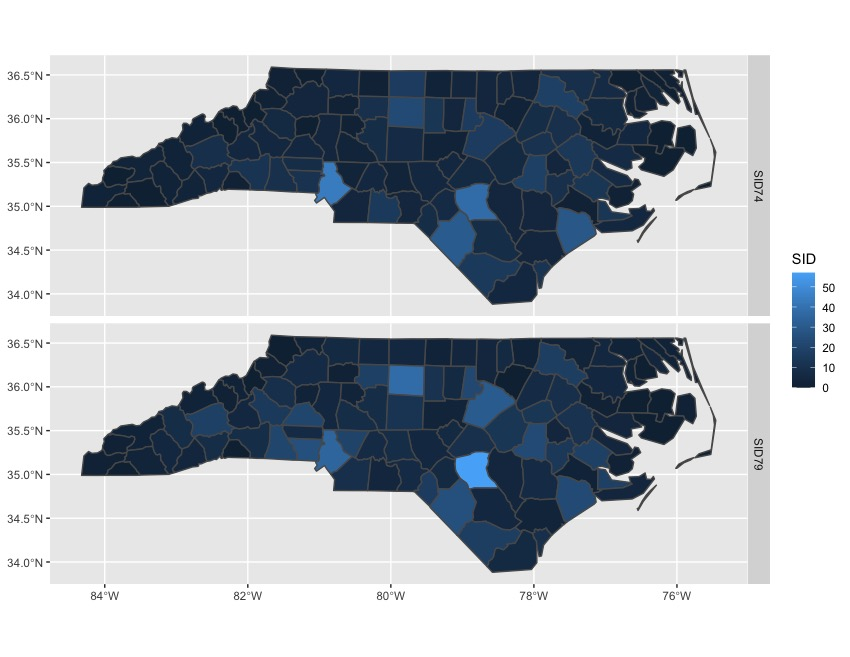
\includegraphics[width=\textwidth]{./images/ncplot}
  \caption{\label{fig:ncplot} Incidence of SIDS in North Carolina.}
\end{figure}

\lipsum[2]

\subsection{Tables}

Tables can also be included with the standard \LaTeX \ table commands, with
references and labels. The thesis class equips the recommended you use the
\texttt{booktabs} library, which includes commands to introduce horizontal
rules in tables.

\begin{table}
  \begin{center}
\caption{\label{tab:example} An Example Table}
\begin{tabular}{lcccccl}
  \toprule
& \multicolumn{3}{c}{$tol=tols$} & \multicolumn{3}{c}{$tol=told$}
\\\cmidrule(lr){2-4}
\cmidrule(lr){5-7}
           & $mv$  & Rel.~err & Time    & $mv$  & Rel.~err & Time\\
\midrule
trigmv    & 11034 & 1.3e-7 & 3.9 & 15846 & 2.7e-11 & 5.6 \\
trigexpmv & 21952 & 1.3e-7 & 6.2 & 31516 & 2.7e-11 & 8.8 \\
trigblock & 15883 & 5.2e-8 & 7.1 & 32023 & 1.1e-11 & 1.4e1\\
expleja   & 11180 & 8.0e-9 & 4.3 & 17348 & 1.5e-11 & 6.6 \\
\bottomrule
\end{tabular}
\end{center}
\end{table}

\subsubsection{Caption Styles}
\lipsum
